\documentclass[useAMS,usenatbib]{mnras}
% A Monthly Notices of the Royal Astronomical Society sample TeX file.
% The teX file has had all publication information removed and been left intentionally blank
\usepackage{graphicx}
\usepackage{float}
\usepackage{graphicx}
\usepackage{psfig}
\usepackage{amsfonts,amssymb,amsmath}
\usepackage{hyperref,color}
\usepackage{textcomp}
\usepackage[T1]{fontenc}
\usepackage{aecompl}
\usepackage{times}
\usepackage[colorinlistoftodos]{todonotes}
\usepackage{txfonts}
\usepackage[english]{babel}
\usepackage[utf8x]{inputenc}
\usepackage{amsmath}
\usepackage{graphicx}
\usepackage{caption}
\usepackage{subcaption}
\usepackage{siunitx}
%\usepackage{booktabs}

\usepackage[colorinlistoftodos]{todonotes}

%\usepackage[authoryear]{natbib}
%\graphicspath{ {images/} }

\def\aap{Astronomy \& Astrophysics}
\def\apj{The Astrophysical Journal}
\def\apjs{The Astrophysical Journal Supplement}
\def\mnras{Monthly Notices of the Royal Astronomical Society}
\def\pasp{Publications of the Astronomical Society of the Pacific}
%
\title{Estimating the probability of causal contact between
civilizations through MonteCarlo simulations}


% Group authors per affiliation:
\author[M. Lares et al.]
{M. Lares\thanks{E-mail: marcelo.lares@unc.edu.ar}\footnotemark[0] $^{1,2,3}$,
J. Funes $^{3, 4}$
\\
% institutions
$^{1}$Instituto de Astronom\'{\i}a Te\'orica y Experimental (CCT C\'ordoba, CONICET, UNC), Argentina.\\
$^{2}$Observatorio Astron\'omico de C\'ordoba, Universidad Nacional de C\'ordoba, Argentina.\\
$^{3}$Consejo Nacional de Investigaciones Cient\'{\i}ficas y
T\'ecnicas, Argentina.\\
$^{4}$Universidad Católica de Córdoba, Argentina
}
%
%\hypersetup{draft}
\begin{document}

\date{Accepted . Received ; in original form }

%\pagerange{\pageref{firstpage}--\pageref{lastpage}} \pubyear{2014}

 \maketitle

\label{firstpage}

\begin{abstract}

\end{abstract}
%
\begin{keywords}
keyword1, keyword2
\end{keywords}
%
%%%%%%%%%%%%%%%%%%%%%%%%%%%%%%%%%%%%%%%%%%%%%%%%%%%%%%%%%%%%%%%%%%%%%%%%%%%%%%%%%%%%
% Introduction
%%%%%%%%%%%%%%%%%%%%%%%%%%%%%%%%%%%%%%%%%%%%%%%%%%%%%%%%%%%%%%%%%%%%%%%%%%%%%%%%%%%%


\section{Motivations: Uncertainties and the non detection problem for
ETI contact}
%{{{


Since the factors in the Drake equation are uncertain, we propose to
avoid the frequentist approach of this equation
and to explore a parameter space, where instead of computing a final
number, we provide a statistical distribution that gives conditional
probabilities.
%
The only fact that can be stated with certainty is that for the number
of years SETI projects have been working we have not received any
signal within the conditions stablished by SETI.



The discrete events method for simulating a stochastic process is an
approximation that allows to study the behaviour of complex
systems, by considering a sequence of well defined discrete events.
%
The simulation os carried out by following all the variables that
describe the system, that constitute the state of the system.
%
The evolution of the process, then, is described as a set of changes
in the state of the system.
%
In this context, an event produces a specific change in the state,
that can be triggered by random variables that encode the stochastic
nature of the physical phenomenon.
%
The process involves following the changes on the state of the system,
definig the initial and final states, defining a method that allows to
keep track of time progress, and maintaining a list of relevant
events.
%}}}


\section{Methods: accounting for causal contacts with 
discrete event simulation process}
%{{{

On the particular case of the difusion of signals of intelligence in
the Galaxy, the discrete events method can be performed taking into
account a small number of variables.  The temporal structure is
defined by two distribution parameters that represent the mean
time interval that an intelligent civilization can emit and receive
signals, and the mean time interval between the emergence of an
intelligent comunicating civilization and the next.
The spatial structure of the simulation is given by the size and shape
of the Galactic Habitable Zone and the maximum distance a signal can
travel to be detected.

Also, some hypothesis must be made in order to complete the
simulation, namely:

\begin{itemize}
   \item The capacity to emit signals and to receive signals ocurr at
      the same time.
   \item All CETIs use the same signal power, so that there is a
      maximum distance out to which it can be detected.
   \item The distribution of the appeareance of new CETIs
      is a stationary Poisson distribution.
   \item The distribution of duration of CETIs
      is a stationary exponential distribution.
   \item There is no a temporal window 
   \item The probability for the rise of a CETI is homogeneous
      over the GHZ.
   \item The message travels at light speed.

\end{itemize}


The fixed variables of the simulation are not explored:


\begin{itemize}
   \item Size of the GHZ
\end{itemize}


The variables that are explored with the simulation are:

\begin{itemize}
   \item Mean number of CETIs (Drake equation), or equivalently, the
      mean time between the awakening of two consecutive CETIs,
      $\tau_N$
   \item Mean lifetime of a CETI, $\tau_a$
   \item Maximum reach of CETI messages, $D_{max}$
\end{itemize}

The main variables that follow the evolution of the simulation are:

\begin{itemize}
   \item Position of stars.  Sampled randomly within the GHZ
   \item Time of the awakening of each CETI
   \item Time of the vanishing of each CETI
\end{itemize}

The variables that can be deduced from the previous ones are:

\begin{itemize}
   \item Number of CETIs in casual contact with at least another CETI
      at a given time.
   \item Number of CETIs as a function of time
   \item Number of CETIs that receive a message at least one time
   \item Number of CETIs that receive a message at least one time and
      successfully deliver an answer.
   \item Number distribution of waiting time to receive a message
\end{itemize}


%========================================================================
%========================================================================
%========================================================================


Possible hypothesis improvements are:

\begin{itemize}
   \item Dmax is different for different CETIs.  For example a power
      law where powerfull emmisions are rare and weak emssions are
      common.
   \item The probability of the rising of a new CETI vary within the
      GHZ.
   \item Correction by coverage ratio in the detection and by
      targetting ratio in the emission.
   \item Spiritual factor.  Explore the role of the S factor: message
      contents, influence on the lifespan of a CETI that receives a
      message, mean lifespan of a CETI that emits a message.
\end{itemize}


\subsection{Model for CETIs}


Since the method is based on events, the first step is to define an
architecture of events, the relationships between them and how events
trigger changes on the state of the system.
%
We consider a simulated system that represents the galactic habitable
zone (GHZ).
%
On a first approach, the GHZ is a 2-dimensional annular region.
%
This simple model does not take into accont the variations in stellar
density given by the spiral structure.
%
Although there are several possible approaches, we chose to follow the
evolution of the system according to the following events:


\begin{enumerate}
   \item[(A)] A new CETI appears (Awakening)
   \item[(D)] An old CETI dissappears (Doomsday)
   \item[(C)] A new causal contact is stablished (Contact)
   \item[(B)] An existing causal contact is interrupted (Blackout)
\end{enumerate}


The event of type B is produced when one of the two CETIs halts in its
capability of emmiting and receiving signals.













%======================================================================
%======================================================================
%======================================================================


The system is updated each time an event is produced.  The time marks
for each event (A and D for each CETI and C and B for each causal
contact) are stored as a result of the simulation.
%
Also, the list of active CETIs is obtained as a function of time.

Some fixed variables must be set in order to carry out the simulation,
namely:

\begin{itemize}
   \item Size of the Galactic Habitable Zone.  Radial symetry is
      assumed, so that the GHZ is determined by two radii, the inner
      radius (GHZ_inner) and the outer radius (GHZ_outer).  They are
      measured in light years, with the aim to maintain y single and
      comprehensive unit for both space and time coordinates.
   \item Mean lifetime of a CETI
   \item Mean waiting time for the appeareance of another CETI
   \item Maximum distance a message can be detected
\end{itemize}


%Variables en el programa
%\begin{itemize}
%   \item Nact: Número de CETIs activas
%   \item Nsee: Número de contactos por cada CETI
%   \item Nccc: CETIs en contacto causal. Notar que una CETI puede tener múltiples
%contactos de otras CETIs. Para cada una de ellas, guardar:
%   \item ID: ID de la CETI emisora
%   \item ID: ID de la CETI receptora
%   \item t\_hola: tiempo del primer contacto
%   \item t\_chau: tiempo del último contacto
%\end{itemize}
%
%
%Caso 1: aparece una nueva CETI
%Modificaciones al estado del sistema:
%\begin{itemize}
%   \item Agregar la CETI “A” a la lista de CETIs activas
%   \item Sortear la duración de la actividad de comunicación de la CETI “A”
%   \item Sortear el intervalo de tiempo hasta la aparición de la próxima CETI:
%t\_WakeUp\_next
%   \item Agregar la CETI “A” al árbol
%   \item Identificar todas las CETIs que están a menos de D max de la nueva CETI, y
%actualizar la lista de tiempos
%\end{itemize}
%
%Caso 2: desaparece una CETI
%Modificaciones al estado del sistema:
%\begin{itemize}
%   \item Eliminar la CETI a la lista de CETIs activas
%\end{itemize}
%
%
%Caso 3: una nueva CETI entra en contacto causal
%Modificaciones al estado del sistema:
%\begin{itemize}
%   \item Agregar la CETI B a la lista de contactos de la CETI A
%\end{itemize}
%


%}}}


\section{Results: exploring the parameter space}
%{{{

As the result of the simulation, several quantities are obtained.


 
%#
%# CONTENTS OF THE <CETIS> PICKLE:
%# . . . . . . . . . . . . . . . . . . . . . . . .
%# 0. ID of emitting CETI
%# 1. ID of emitting [receiving] CETI
%# 2. x position in the galaxy
%# 3. y position in the galaxy
%# 4. time of Awakening [Contact]
%# 5. time of Doomsday  [Blackout]
%# . . . . . . . . . . . . . . . . . . . . . . . .
%#
%# This structure is always for the A-D cycle of each emitting CETI,
%# and repeats for each contact (C-B).
%#
%# The time span of a CETI is t_D - t_A for CETIs[k][0]
%# The time span of a contact is t_B - t_C for CETIs[k][i], with i>0
%#
%#
%# age: time elapsed from A to a given time
%# ceti_e: ceti emitting signals (emiter)
%# ceti_r: ceti receiving signals (receiver)
%# ceti_c: ceti that listen at least another ceti (citizen)
%# ceti_h: ceti that is lestened by at least another ceti
%#
%
%# for Check purposes
%#-------------------
%# duration of a civilization (exponential distribution by costruction)
%# time from the appeareance of a CETI to the next
%#
%# 
%# derived quantities
%#-------------------
%# [time]
%# time span of a ceti listening another
%# time span of a ceti being listened by another
%# duration of two-way communication channels
%# waiting time until the first contact
%# fraction of awaken time a ceti is listening at least another ceti
%# age of contacted cetis_e at first C
%# distribution of time to wait until next C
%# fraction of cetis where the first contact is given at the A
%
%# [numbers]
%# distribution of the number of contacts for each ceti
%# distribution of the maximum number of contacts for each ceti
%# distribution of the number of contacts as a function of age
%# number of contacts as a function of time in the galaxy
%# rate of cetis that succeed in contact 
%# fraction of contacts that admit a response
%#
%# [distances]
%# distribution of distances between contacted cetis
%#
%# [correlations] relation between {RB}
%# RB distance to ceti and time of double communication
%# RB distance to ceti and age of contacted ceti
%# RB the age of a ceti and the maximum number of contacted cetis before D
%# RB lifespan of a ceti and max number of contacts
%#
%# distribution in the galaxy of cetis that reach contact
%
%# ... everything as a function of parameters!    





Output
\begin{itemize}
   \item La salida de la simulación está guardad en una variable llamada CETI.
   \item La misma es una lista de objetos que son también listas.
   \item El elemento cero de cada lista (i.e., cada elemento de CETI) contiene:
   \item coordenada X
   \item coordenada Y
   \item tiempo de inicio de la capacidad de comunicación
   \item tiempo de final de la capacidad de comunicación
   \item y los demás elementos contienen:
   \item coordenada X de la CETI
   \item coordenada Y de la CETI
   \item tiempo del primer contacto
   \item tiempo del último contacto
\end{itemize}

%}}}


\section{Results}
%{{{

Resultados cuantitativos de la simulación
\begin{itemize}
   \item distribucion del numero de contactos
   \item distribucion de la duracion de los contactos
   \item distribucion del tiempo que hay que esperar para el proximo contacto
\end{itemize}



\begin{figure}
   \centering
   \includegraphics[width=0.5\textwidth]{growingsphere.pdf}
   \caption{Schematic representation of the growing communicating
   sphere, over the space--time diagrams.  In (a) the sphere is
   growing as the surface of first contact has not reached the maximum
   distance.  In (b) it has reached the maximum distance, so that it
   remains at the same size.  After a Doomsday event, the signals can
   still be observed, but the surface of last contact grows }
   \label{F_sphere}
\end{figure}

  
\begin{figure}
   \centering
   \includegraphics[width=0.5\textwidth]{abcd.pdf}
   \caption{Schematic representation of two emitters, $E_1$ and $E_2$,
   that reach each other at different times.  The time span for $E_i$
   is $(A_i, D_i)$, for $i=\{1,2\}$.  Emitter $i$ can listen to
   emitter $j$ between $C_{ij}$ and $B_{ij}$.
   The type and length of causal contact in both directions depend on
   the distance and time lag between the awakening events, the maximum
   distance that a signal can reach and the time period in which each
   emitter is active.}
   \label{F_abcd}
\end{figure}

 
 
\begin{figure*}
   \centering
   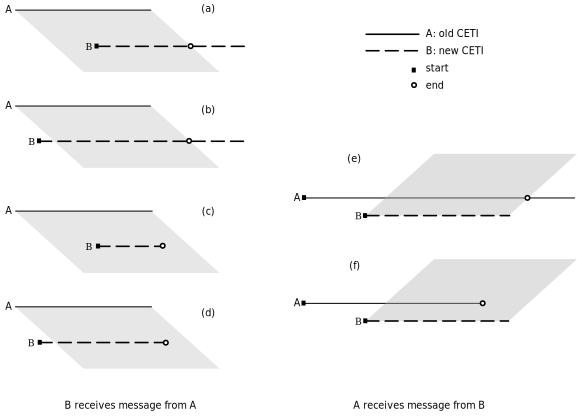
\includegraphics[width=\textwidth]{Messages_01.pdf}
   \caption{Schematic representation of the possible cases in which a
   ceti A can be in causal contact with a ceti B which appears later.
   The duration of the causal contact in one direction depends on
   several factors, mainly $\Delta t_A$, $\Delta t_C$, and $\Delta X$.}
   \label{F_messages}
\end{figure*}

 




Posibles implicaciones
\begin{itemize}
   \item Análisis del método de comunicación: isotrópico, colimado, accidental
   \item Naturaleza del transporte del mensaje: radiación electromagnética u otros
   \item Efectos de fenómenos de alineación (tránsitos)
   \item Marcadores energéticos
   \item Marcadores espirituales
   \item Uso de estrellas como amplificadores o fuentes
\end{itemize}

%}}}



Under the hypotheses of our experiments, we conclude that
a causal contact is extremely unlikely unless the Galaxy is heavily
populated by intelligent civilizations.
%
Even so, we must consider that in order to stablish a contact between
any two entities, a minimum degree of compatibility must be
accomplished without any previous agreement, 
making the posibility of a contact with a message that
could be deciphered highly rare.
 


\bibliographystyle{mn2e}
\bibliography{biblio_seti}
\end{document}
